\documentclass[]{../template/Report}%方括号内写yuxi即生成预习报告\documentclass[yuxi]{../template/Report}
\settemplatedir{../template/}%设置模板路径

\exname{等厚干涉} %实验名称
\extable{14} %实验桌号
\instructor{张利} %指导教师
\class{信工2401} %班级
\name{姚舜瑜} %姓名
\stuid{3240100532} %学号

\nyear{2025} %年
\nmonth{12} %月
\nday{2} %日
\nweekday{二} %星期几，e.g. \nweekday{三}
\daypart{上午}%上午/下午

\redate{} %如有实验补做，补做日期
\resitu{} %情况说明：

\begin{document}
\maketitle%输出封面

\section{预习报告（10分）}
\subsection{实验综述（5分）}

\subsubsection{实验目的}
\begin{enumerate}
  \item 通过观察牛顿环和劈尖干涉条纹，直观熟悉等厚干涉现象，理解膜厚与条纹级次之间的对应关系。
  \item 学会利用牛顿环测量凸透镜曲率半径、利用劈尖条纹测量薄片厚度的基本步骤和数据处理方法。
  \item 练习读数显微镜的使用，体会单向读数、减小空程误差和估计不确定度在精密测量中的作用。
\end{enumerate}

\subsubsection{背景与原理}
等厚干涉是一种经典的光学干涉现象，产生于两块光滑透明介质之间的薄膜。当单色光近垂直入射时，薄膜中不同位置的膜厚决定了反射光的光程差，从而形成明暗相间的干涉条纹。由于膜厚在空间上分布不均匀，不同位置对应不同的干涉级次，形成等厚干涉图样。

本实验属于反射式等厚干涉：两光滑界面之间形成的薄膜中，只要局部膜厚相同，反射光的光程差就相同，从而得到同一级条纹。近垂直入射单色光时，上下表面反射光的光程差为
\[
\Delta = 2e + \frac{\lambda}{2},
\]
其中 $e$ 为膜厚，$\lambda/2$ 表示一次反射导致的半波相位变化。反射暗纹满足
\[
\Delta = k\lambda,\quad k=0,1,2,\dots
\]

以此为基础，便可以解释两种典型的等厚干涉现象：牛顿环与劈尖干涉。并根据理论推理和测量结果得到目标物理量。

\paragraph{\textbf{1. 牛顿环：}}
\paragraph{}
将曲率半径为 $R$ 的凸透镜轻放在平板玻璃上，在接触附近形成很薄的空气层。几何关系表明，当 $r\ll R$ 时，距中心半径为 $r$ 处的空气层厚度近似
\[
e \approx \frac{r^2}{2R},
\]
代入暗纹条件可得第 $k$ 级暗环
\[
r_k^2 = kR\lambda.
\]
因此 $r_k^2$ 与条纹级次 $k$ 近似成线性关系。实际处理中常取两级暗环平方差
\[
r_m^2 - r_n^2 = (m-n)R\lambda,
\]
从而计算
\[
R = \frac{r_m^2 - r_n^2}{(m-n)\lambda}
  = \frac{\Delta d^2}{4(m-n)\lambda},
\]
以减弱中心定位和单次读数误差的影响。


\paragraph{\textbf{2. 劈尖干涉：}}
\paragraph{}

用两块玻璃片与待测薄片在一端组成空气劈尖，沿劈尖方向膜厚近似线性变化。相邻同种条纹对应的膜厚差约为 $\lambda/2$。若在长度为 $L$ 的一段劈尖上共数到 $N$ 条条纹，则薄片厚度
\[
e = \frac{\lambda N}{2} = \frac{\lambda nL}{2},
\]
其中 $n$ 为单位长度内的条纹条数。为减小读数误差，通常利用跨越 10 条纹的平均条距
\[
\overline{\Delta S}_{10} = \frac{1}{10}\sum_{i=1}^{10}(S_{i+10} - S_i),\quad
n = \frac{10}{\overline{\Delta S}_{10}},
\]
于是得到
\[
e = \frac{50L\lambda}{\sum_{i=1}^{10}(S_{i+10} - S_i)}.
\]
最终结果写成 $e = \bar e \pm u_e$ 的形式，并说明主要不确定度来源。

\begin{figure}[H]
  \centering
  \begin{minipage}{0.45\textwidth}
    \centering
  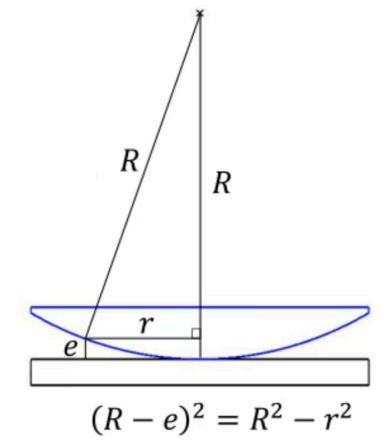
\includegraphics[width=0.8\textwidth]{figures/仪器示意图.png}
  \caption{牛顿环原理示意图}
  \end{minipage}
  \hfill
  \begin{minipage}{0.45\textwidth}
    \centering
  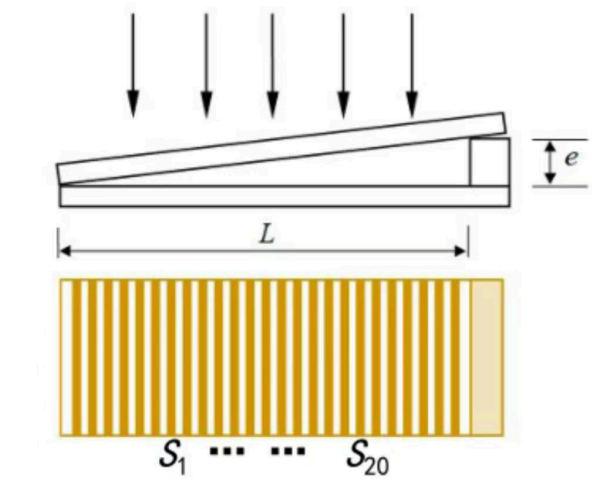
\includegraphics[width=\textwidth]{figures/条纹示意图.png}
  \caption{劈尖干涉原理示意图}
  \end{minipage}
\end{figure}
\subsubsection{实验仪器}
钠灯；读数显微镜；光学平板玻璃和凸透镜（牛顿环装置）；两块平玻璃片与待测薄片（劈尖干涉装置）；半反半透镜等。

\subsubsection{实验内容}
\begin{enumerate}
  \item \textbf{读数显微镜调节：}先调节目镜使十字丝清晰，再调物镜使条纹成像锐利，移动视线检查并消除视差。
  \item \textbf{牛顿环实验：}搭建牛顿环装置，调整透镜与平板的接触和水平度，使同心环清晰。用读数显微镜沿固定方向单向转动测微鼓轮，记录若干级左右暗环位置，计算各级半径 $r_k$，建立 $r_k^2$–$k$ 关系，拟合得到凸透镜曲率半径 $R$。
  \item \textbf{劈尖测厚实验：}搭建劈尖干涉装置，微调劈尖角度和显微镜焦距，使直条纹细而清晰。选取包含薄片的一段长度 $L$，多次记录条纹坐标（如 $S_i$ 与 $S_{i+10}$），求出平均条距和条纹密度 $n$，代入公式计算薄片厚度，并结合重复测量结果估算不确定度。
\end{enumerate}

\subsection{实验重点（3分）}

\begin{itemize}
  \item 理解等厚干涉原理，掌握牛顿环和劈尖干涉的形成机制及其与膜厚的关系。
  \item 熟练使用读数显微镜，掌握单向读数和减小空程误差的方法。
  \item 能结合实验数据进行合理的数据处理和不确定度分析。
\end{itemize}

\subsection{实验难点（2分）}

\begin{itemize}
  \item 牛顿环中心及高阶条纹对比度较低，中心位置与条纹级次判定容易产生偏差。
  \item 读数显微镜存在回程间隙，若未严格单向读数，易引入系统性空程误差。
  \item 劈尖条纹细密，对显微镜对焦、劈尖平行度和光路垂直度要求较高，稍有偏差就会导致条纹模糊、计数困难。
\end{itemize}
\begin{fullreportonly}
\section{原始数据（20分）}
\begin{figure}[H]
  \centering
  
\includegraphics[width=0.8\textwidth]{figures/原始数据.jpg}
  \caption{实验原始数据记录示例}
\end{figure}
\newpage
\section{结果与分析（60分）}
\subsection{数据处理与结果（30分）}
\subsubsection{牛顿环实验结果}
\begin{table}[H]
  \centering
  \caption{牛顿环数据记录与处理}
  \begin{tabular}{ccccc}
    \toprule
    条纹级次 $k$ & $d_{\text{左}}$ (mm) & $d_{\text{右}}$ (mm) & 直径 $d_k$ (mm) & $d_k^2$ ($mm^2$) \\
    \midrule
    10 & 15.740 & 10.610 & 5.130 & 26.3169 \\
    9  & 15.630 & 10.720 & 4.910 & 24.1081 \\
    8  & 15.490 & 10.850 & 4.640 & 21.5296 \\
    7  & 15.340 & 10.995 & 4.345 & 18.8790 \\
    6  & 15.195 & 11.130 & 4.065 & 16.5242 \\
    5  & 15.040 & 11.295 & 3.745 & 14.0250 \\
    4  & 14.855 & 11.470 & 3.385 & 11.4582 \\
    3  & 14.660 & 11.675 & 2.985 & 8.9102 \\
    2  & 14.410 & 11.930 & 2.480 & 6.1504 \\
    1  & 14.125 & 12.155 & 1.970 & 3.8809 \\
    \bottomrule
  \end{tabular}
\end{table}
通过逐差法计算（取 $m-n=5$），得到各组 $d_m^2 - d_n^2$ 及对应的曲率半径 $R$ 如下（已知 $\lambda = 589.3\,\text{nm}$）：
\begin{table}[H]
  \centering
  \caption{逐差法计算曲率半径 $R$}
  \begin{tabular}{cc}
    \toprule
    \textbf{相隔5圈直径平方数之差} ($\text{mm}^2$) & \textbf{R} (m) \\
    \midrule
    $d_{10}^2 - d_5^2 = 12.2919$ & 1.043 \\
    $d_{9}^2 - d_4^2 = 12.6499$ & 1.073 \\
    $d_{8}^2 - d_3^2 = 12.6194$ & 1.071 \\
    $d_{7}^2 - d_2^2 = 12.7286$ & 1.080 \\
    $d_{6}^2 - d_1^2 = 12.6433$ & 1.073 \\
    \bottomrule
  \end{tabular}
\end{table}
根据结果可知，取平均值作为最终结果：
\[\overline{R} = \frac{1.043+1.073+1.071+1.080+1.073}{5} =1.072 \,\text{m}.\]



\subsubsection{劈尖干涉实验结果}
根据测量得到劈尖的左侧边界$L_{\text{左}}=38.740(mm)$，右侧边界$L_{\text{右}}=-0.063(mm)$，计算劈尖长度为：
\[L=L_{\text{左}}-L_{\text{右}}=38.803(mm).\]
利用下表数据计算各组 $S_{i+10} - S_i$：
\begin{table}[H]
  \centering
  \caption{劈尖干涉数据记录与处理}
  \begin{tabular}{cccc}
    \toprule
    条纹编号 $i$ & $S_i$ (mm) & $S_{i+10}$ (mm) & $S_{i}-S_{i+10}$ (mm) \\
    \midrule
    1 & 28.000 & 25.750 & 2.250 \\
    2 & 27.790 & 25.549 & 2.241 \\
    3 & 27.385 & 25.110 & 2.275 \\
    4 & 27.360 & 25.070 & 2.290 \\
    5 & 27.160 & 24.844 & 2.316 \\
    6 & 26.910 & 24.562 & 2.348 \\
    7 & 26.680 & 24.345 & 2.335 \\
    8 & 26.650 & 24.320 & 2.330 \\
    9 & 26.230 & 23.890 & 2.340 \\
    10 & 26.005 & 23.755 & 2.250 \\
    \bottomrule
  \end{tabular}
\end{table}
计算得到：
\[\sum_{i=1}^{10}(S_{i+10} - S_i) = 22.975(mm).\]
代入薄片厚度公式：
\[e = \frac{50L\lambda}{\sum_{i=1}^{10}(S_{i+10} - S_i)} = \frac{50 \times 38.803 \times 0.5893}{22.975} = 49.78 (\mu m).\]

\subsection{误差分析（20分）}

\subsubsection{牛顿环曲率半径 $R$ 的不确定度}
根据逐差法计算得到的 5 组 $R$ 值：1.043, 1.073, 1.071, 1.080, 1.073 (m)。
平均值：
\[ \overline{R} = \frac{1}{5}\sum_{i=1}^5 R_i = 1.068 \, \text{m} \]
A 类不确定度（标准偏差）：
\[ u_A(R) = \sqrt{\frac{\sum_{i=1}^5 (R_i - \overline{R})^2}{5(5-1)}} = \sqrt{\frac{0.000828}{20}} \approx 0.0064 \, \text{m} \]
假设 B 类不确定度主要来自仪器读数误差，相比 A 类分量较小，故取合成不确定度 $u_c(R) \approx u_A(R) = 0.006 \, \text{m}$。
最终结果：
\[ R = \overline{R} \pm u_c(R) = 1.068 \pm 0.006 \, \text{m} \quad \]
相对不确定度：
\[ E_R = \frac{u_c(R)}{\overline{R}} \times 100\% = \frac{0.006}{1.068} \times 100\% \approx 0.6\% \]

\subsubsection{劈尖薄片厚度 $e$ 的不确定度}
10 个条纹间距差值 $\Delta S_i = S_i - S_{i+10}$ 的平均值：
\[ \overline{\Delta S} = \frac{1}{10} \sum_{i=1}^{10} \Delta S_i = 2.2975 \, \text{mm} \]
其 A 类不确定度：
\[ u_A(\Delta S) = \sqrt{\frac{\sum (\Delta S_i - \overline{\Delta S})^2}{10(10-1)}} \approx 0.013 \, \text{mm} \]
劈尖长度 $L$ 的测量不确定度设为 $u(L)$，假设相对误差较小。
根据公式 $e = \frac{50 L \lambda}{\sum \Delta S_i} = \frac{5 L \lambda}{\overline{\Delta S}}$，忽略 $\lambda$ 的误差，相对不确定度合成公式为：
\[ \frac{u(e)}{e} = \sqrt{\left(\frac{u(L)}{L}\right)^2 + \left(\frac{u(\overline{\Delta S})}{\overline{\Delta S}}\right)^2} \]
其中 $\frac{u(\overline{\Delta S})}{\overline{\Delta S}} = \frac{0.013}{2.2975} \approx 0.57\%$。若忽略 $L$ 的误差，则 $u(e) \approx e \times 0.57\% \approx 49.78 \times 0.0057 \approx 0.28 \, \mu\text{m}$。
最终结果：
\[ e = 49.78 \pm 0.28 \, \mu\text{m} \]

\subsubsection{误差原因分析}
\begin{enumerate}
    \item \textbf{读数误差：} 显微镜读数时十字丝对准条纹中心的判断存在主观偏差，且条纹本身具有一定宽度，导致读数分散。
    \item \textbf{空程误差：} 尽管实验中要求单向转动鼓轮，但若中途有微小反转或机械间隙未完全消除，会引入系统误差。
    \item \textbf{样品状态：} 牛顿环透镜与平板接触点可能有微尘，导致接触斑变大或变形；劈尖玻璃片表面平整度及薄片厚度的均匀性也会影响条纹的等间距性。
    \item \textbf{条纹级次判断：} 在牛顿环中心暗斑模糊或劈尖条纹密集时，级次计数可能出错。
\end{enumerate}
\subsection{实验探讨（10分）}
通过本次实验，我们成功利用等厚干涉现象测量了凸透镜的曲率半径和薄片的厚度。从理论层面上，我对光学中的干涉原理有了更深入的理解，尤其是等厚干涉中膜厚与干涉级次之间的关系。
在实验层面上，我体会到了精密测量中读数显微镜的使用技巧，如单向读数和减小空程误差的重要性。此外，我也学会了在数据处理过程中使用逐差法减小系统误差，提高了结果的准确性。

\section{思考题（10分）}
\subsection{如果读数显微镜的叉丝不是准确地通过圆心，那么测出的直径实际上是弦长，这对测量结果有无影响？并解释原因}
\paragraph{答：}如果读数显微镜的叉丝没有准确通过圆心，测得的实际上是弦长而非直径。但是在本实验中我们采用的是逐差法公式：
\[R = \frac{d_m^2 - d_n^2}{4(m-n)\lambda}\]
假设叉丝偏离圆心的距离为 $h$，则测得的弦长 $l_k$ 与真实直径 $d_k$ 的关系为：
\[l_k^2 = d_k^2 - 4h^2\]。
代入逐差法公式计算：
\[
\frac{l_m^2 - l_n^2}{4(m-n)\lambda} = \frac{(d_m^2 - 4h^2) - (d_n^2 - 4h^2)}{4(m-n)\lambda} = \frac{d_m^2 - d_n^2}{4(m-n)\lambda}.
\]
可以看到，常数项 $4h^2$ 在相减过程中被消去，最终结果和原公式没有区别。因此，只要偏离距离 $h$ 保持不变（即显微镜移动轨迹是一条直线），测量弦长而非直径\textbf{不会影响}曲率半径 $R$ 的测量结果。

\subsection{反射光干涉观察到牛顿环中央是暗斑，那么从透射方向观察，牛顿环中央是暗斑还是亮斑？}
\paragraph{答：}从透射方向观察牛顿环时，中央会是亮斑。这是因为反射光与透射光的干涉条件互补。
对于反射光，由于在空气-玻璃界面反射时存在半波损失，其光程差为：
\[ \Delta_R = 2e + \frac{\lambda}{2} \]
在中心接触点处膜厚 $e \approx 0$，此时 $\Delta_R = \lambda/2$，满足干涉相消条件，故呈现暗斑。
而对于透射光，其光程差不包含半波损失（或可视作两次反射引入 $2 \times \frac{\lambda}{2} = \lambda$ 的相位变化），即：
\[ \Delta_T = 2e \]
在中心接触点处 $e \approx 0$，此时 $\Delta_T = 0$，满足干涉相长条件：
\[ \Delta = k\lambda \quad (k=0) \]
因此，透射方向观察到的牛顿环中央是亮斑。
\end{fullreportonly}
\insertnotes
\end{document}
